\documentclass[a4paper,11pt]{article}
\usepackage[slovene]{babel}
\usepackage[utf8]{inputenc}
\usepackage{graphicx}
\usepackage{hyperref}
\usepackage{listings}
\usepackage{geometry}
\geometry{margin=1in}

\title{\textbf{Extreme Weather Event Notifier}}
\author{Skupina 2425}
\date{\textbf{2025}}

\begin{document}

\maketitle

\newpage

\section*{Povezava do repozitorija kode}
Projektna koda je dostopna na javno dostopnem repozitoriju GitHub, kar omogo\v{c}a vpogled v implementacijo ter CI/CD konfiguracijo:
\begin{itemize}
    \item Repozitorij: \url{https://github.com/rso2425/extreme-weather-event-notifier}
    \item Aplikacija: \url{https://rso-weather.duckdns.org/}
\end{itemize}

\section*{Kratek opis projekta}
Extreme Weather Event Notifier je spletna aplikacija, ki uporabnike obve\v{s}\v{c}a o ekstremnih vremenskih dogodkih v Sloveniji. Uporabniki lahko omogo\v{c}ijo prejemanje potisnih obvestil in dostopajo do zgodovine vremenskih dogodkov. Aplikacija zbira podatke iz Agencije Republike Slovenije za okolje (ARSO) in jih obdeluje v mikrostoritvenem sistemu. Potisna obvestila se po\v{s}iljajo preko Firebase Cloud Messaging, podatki pa se shranjujejo v MongoDB in so dostopni preko spletnega vmesnika.

\section*{Ogrodje in razvojno okolje}
Pri razvoju projekta so bili uporabljeni sodobni jeziki in orodja, ki omogo\v{c}ajo skalabilno in vzdr\v{z}evalno infrastrukturo:
Frontend je implementiran s pomo\v{c}jo Vue.js, za backend pa se uporablja Express.js. Podatki se shranjujejo v MongoDB, medtem ko RabbitMQ slu\v{z}i za medstoritveno komunikacijo. Infrastruktura temelji na Dockerju in Kubernetesu, CI/CD procesi pa so avtomatizirani s pomo\v{c}jo GitHub Actions.
\newpage
\section*{Arhitektura sistema}
Arhitektura aplikacije temelji na mikrostoritvenem modelu, kjer vsaka storitev izpolnjuje dolo\v{c}eno funkcijo:
\begin{figure}[h!]
    \centering
    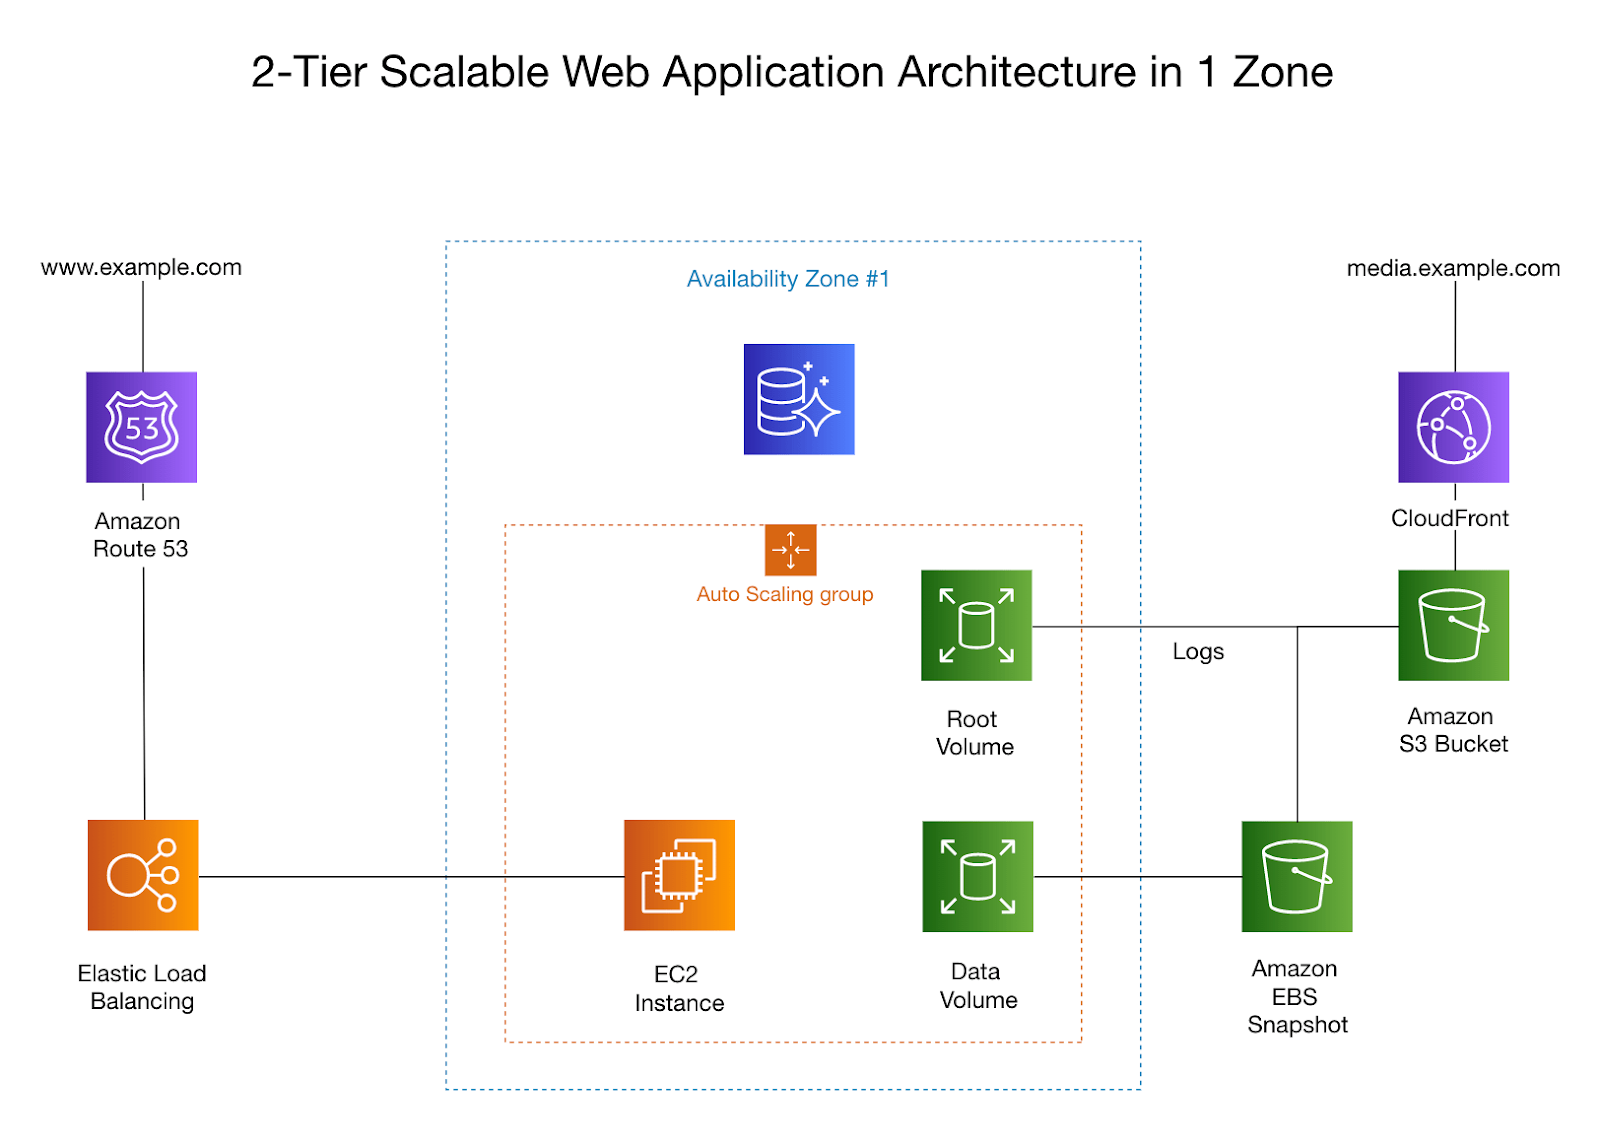
\includegraphics[width=\textwidth]{architecture_diagram.png}
    \caption{Shema arhitekture aplikacije}
\end{figure}

Aplikacija sestavljajo \v{s}tiri glavne mikrostoritve: Web (frontend), Notification, Scraper in Storage. Komunikacija med storitvami poteka preko RabbitMQ in API-jev (REST in GraphQL). Push obvestila se po\v{s}iljajo preko Firebase Cloud Messaging.

\section*{Opis mikrostoritev}
\subsection*{Web Microservice (Frontend)}
Web mikrostoritev predstavlja uporabni\v{s}ki vmesnik aplikacije, implementiran v Vue.js. Uporabnikom omogo\v{c}a:

- Pregled zgodovine vremenskih dogodkov, ki se pridobijo iz Storage mikrostoritve preko GraphQL.

- Prijavo in odjavo na potisna obvestila preko Notification mikrostoritve.

- Upravljanje potisnih obvestil s Firebase Cloud Messaging.

\subsection*{Notification Microservice}
Notification mikrostoritev je odgovorna za po\v{s}iljanje potisnih obvestil in upravljanje Firebase ID-jev uporabnikov. Prejema dogodke iz Scraper mikrostoritve preko RabbitMQ in po\v{s}ilja obvestila uporabnikom z registriranimi napravami.

\subsection*{Scraper Microservice}
Scraper mikrostoritev periodi\v{c}no zbira podatke o vremenskih dogodkih iz ARSO preko CAP XML standarda. Ti podatki se obdelujejo in po\v{s}iljajo Notification ter Storage mikrostoritvama preko RabbitMQ.

\subsection*{Storage Microservice}
Storage mikrostoritev shranjuje podatke o vremenskih dogodkih v MongoDB in izpostavlja GraphQL API, ki omogo\v{c}a pridobivanje podatkov za prikaz zgodovine dogodkov v Web mikrostoritvi.

\section*{CI/CD in testiranje}
CI/CD proces je implementiran s pomo\v{c}jo GitHub Actions. Vklju\v{c}uje:

- Za\v{s}\v{c}ito glavne veje "main", kjer so spremembe mo\v{z}ne le preko pull requestov.

- Avtomatizirano gradnjo in testiranje Docker slik.

- Name\v{s}\v{c}anje posodobljenih slik v Kubernetes preko DigitalOcean Container Registry.

Testiranje je razdeljeno na enotne teste za posamezne storitve, integracijske teste za preverjanje komunikacije med storitvami in ro\v{c}no testiranje uporabni\v{s}kega vmesnika.

\section*{Primeri uporabe}
Aplikacija omogo\v{c}a uporabniku enostavno interakcijo:
Uporabnik obi\v{s}\v{c}e spletno mesto, omogo\v{c}i potisna obvestila, in prejme Firebase ID, ki je shranjen v Notification mikrostoritvi. Scraper zazna vremenski dogodek, ki se po\v{s}lje v RabbitMQ. Notification po\v{s}lje obvestilo uporabnikom, Storage pa omogo\v{c}a vpogled v zgodovino dogodkov.

\section*{Zaklju\v{c}ek}
Extreme Weather Event Notifier predstavlja zanesljiv sistem za obve\v{s}\v{c}anje o ekstremnih vremenskih dogodkih. S svojo mikrostoritveno arhitekturo omogo\v{c}a prilagodljivost, raz\v{s}irljivost in enostavno vzdr\v{z}evanje. Projekt uspe\v{s}no naslavlja potrebo po hitrih in zanesljivih informacijah o vremenskih nevarnostih.

\section*{Reference}
\begin{itemize}
    \item Repozitorij projekta: \url{https://github.com/rso2425/extreme-weather-event-notifier}
    \item Aplikacija: \url{https://rso-weather.duckdns.org/}
    \item Firebase Cloud Messaging: \url{https://firebase.google.com/docs/cloud-messaging}
    \item Kubernetes Dokumentacija: \url{https://kubernetes.io/docs/}
    \item ARSO: \url{https://www.arso.gov.si/}
\end{itemize}

\end{document}
